\newcommand{\usedspecs}[5]{
\begin{table}[h!]
\centering
\begin{tabular}{|c||c|} 
 \hline
 Interface & #1 \\
 \hline
 Sample rate & #2 \\ 
 \hline
 Data & #3 \\ 
 \hline
\end{tabular}
\caption{#4. Used technical specifications}
\label{table:#5_specs}
\end{table}
}

\chapter{Implementation}
\label{ch:Implementation}

\section{Hardware}
\label{sec:hardware}

Based on previous research a set of devices and sensors was selected. The selection was done with a goal in mind: to utilize the maximum of the \emph{available space} on a human head and neck. Assuming that those surfaces will allow the recording of the vibrations and movements generated by the jaw movements. 

A Raspberry Pi 3 B+ (RPI) was used a the central processing unit. It has a Bluetooth antenna as well as a variety of wired connectivity options to ease the build of this prototype. As discussed later in \ref{sec:software} the RPI was used not only for the data collection, but as well for the real-time data visualization. The RPI had some hardware limitations to read the raw data directly from some of the sensors. It was solved by using external microcontrollers, see \ref{subsub:bno}, \ref{subsub:emg}.

\subsection{Peripherals}

\begin{table}[h!]
\centering
\begin{tabular}{|>{\raggedright}m{0.25\linewidth}|>{\centering}m{0.1\linewidth}|m{0.3\linewidth}|m{0.25\linewidth}|} 
 \hline
 Device & Amount & Sensor & Area of contact \\ [0.5ex] 
 \hline\hline
 eSense earables \ref{subsub:esense} & 2 & 6 DOF IMU & In ear \\ 
 \hline
 Arduino BNO055 \ref{subsub:bno} & 2 & 9 DOF IMU & Back side of the jaw \\ 
 \hline
 Olimex EMG-Shield & 4 & Electromyography (EMG) & Masseter and temporalis muscles \\ 
 \hline
 Throat microphone & 1 & Vibration sensor & Neck \\ 
 \hline
 Grove GSR & 1 & Galvanic skin response (GSR) & Index and middle finger \\ 
 \hline
\end{tabular}
\caption{Used sensors}
\label{table:used_sensors}
\end{table}

\subsubsection{eSense earables}
\label{subsub:esense}

\begin{figure}[h!]
\centering
\includegraphics[width=0.5\textwidth]{src/media/hardware/esense.png}
\caption{eSense earable \cite{min2018exploring, kawsar2018earables}}
\label{image:esense}
\end{figure}

The eSense earables are a pair of true wireless earphones. The data we are interested in is the 6 DOF IMU located only in the left earpiece only. Because of this limitation two left earpieces were used. Even though the left and right ear pieces are not interchangeable, the participants in the user study didn't notice any difference in the fit in the right ear.

The default frequency of sending of the IMU data is set to 10Hz. Because in this research we are interested solely in the readings from the IMU (no audio playback) it is possible to increase the frequency to up to 100Hz \cite{esense_ble_specification}.

The connection was done directly with the RPI by using a python package called \texttt{bleak}.

\usedspecs{BLE}{100Hz}{Accelerometer \& gyroscope}{eSense earable}{esense}

\subsubsection{Arduino BNO055}
\label{subsub:bno}

\begin{figure}[h!]
\centering
\includegraphics[width=0.5\textwidth]{src/media/hardware/bno.jpg}
\caption{Arduino BNO055 breakout board}
\label{image:bno}
\end{figure}

This (fig. \ref{image:bno}) small breakout board from Arduino has a BNO055, a 9 DOF IMU with sensor fusion on the chip. The fastest of the available protocols for data transmission is I2C. Fortunately the BNO055 has an \texttt{ADR} pin, which if set to high will change its I2C address. It allows the communication with both of the used BNO055s over the same I2C bus.

Even though the RPI has pins for the I2C communication, it doesn't support clock stretching. Using the RPI the collected data was at a much lower frequency (around 30Hz) and generally the connection was unreliable.

After testing different microcontrollers, the decision was made to use the Adafruit Feather HUZZAH ESP8266 board, to read the raw data from the BNO055s and then send it directly to the RPI. Because the RPI couldn't handle reliably more than 2 BLE connections at the same time, the IMU data was transmitted over the Serial Protocol (USB).

\usedspecs{Serial}{100Hz}{Accelerometer \& gyroscope \& quaternion}{Arduino BNO055 in combination with Feather Huzzah}{esense}

\begin{figure}[h!]
\centering
\includegraphics[width=0.5\textwidth]{src/media/hardware/real-bno.png}
\caption{Prototype of Arduino BNO055 with Feather Huzzah}
\label{image:real-bno}
\end{figure}

\subsubsection{Olimex EMG-Shield}
\label{subsub:emg}

\begin{figure}[h!]
\centering
\includegraphics[width=0.5\textwidth]{src/media/hardware/emg.jpg}
\caption{Olimex EMG-Shield}
\label{image:emg}
\end{figure}

The EMG-Boards from Olimex can be stacked on top of each other, to allow readings from up to 6 channels at the same time. To capture the EMG signals from the left and right masseter muscles as well as from the left and right temporalis muscles, 4 EMG-Shields were used. The raw data from the board is analog, so an analog-to-digital (ADC) converter was needed, because the RPI doesn't have any analog input pins. For this purpose the Arduino Uno was used. The collected data was sent directly to the RPI over the Serial Protocol (USB).

\usedspecs{Serial}{256Hz}{EMG}{Olimex EMG-Shield in combination with Arduino Uno}{emg}

\begin{figure}[h!]
\centering
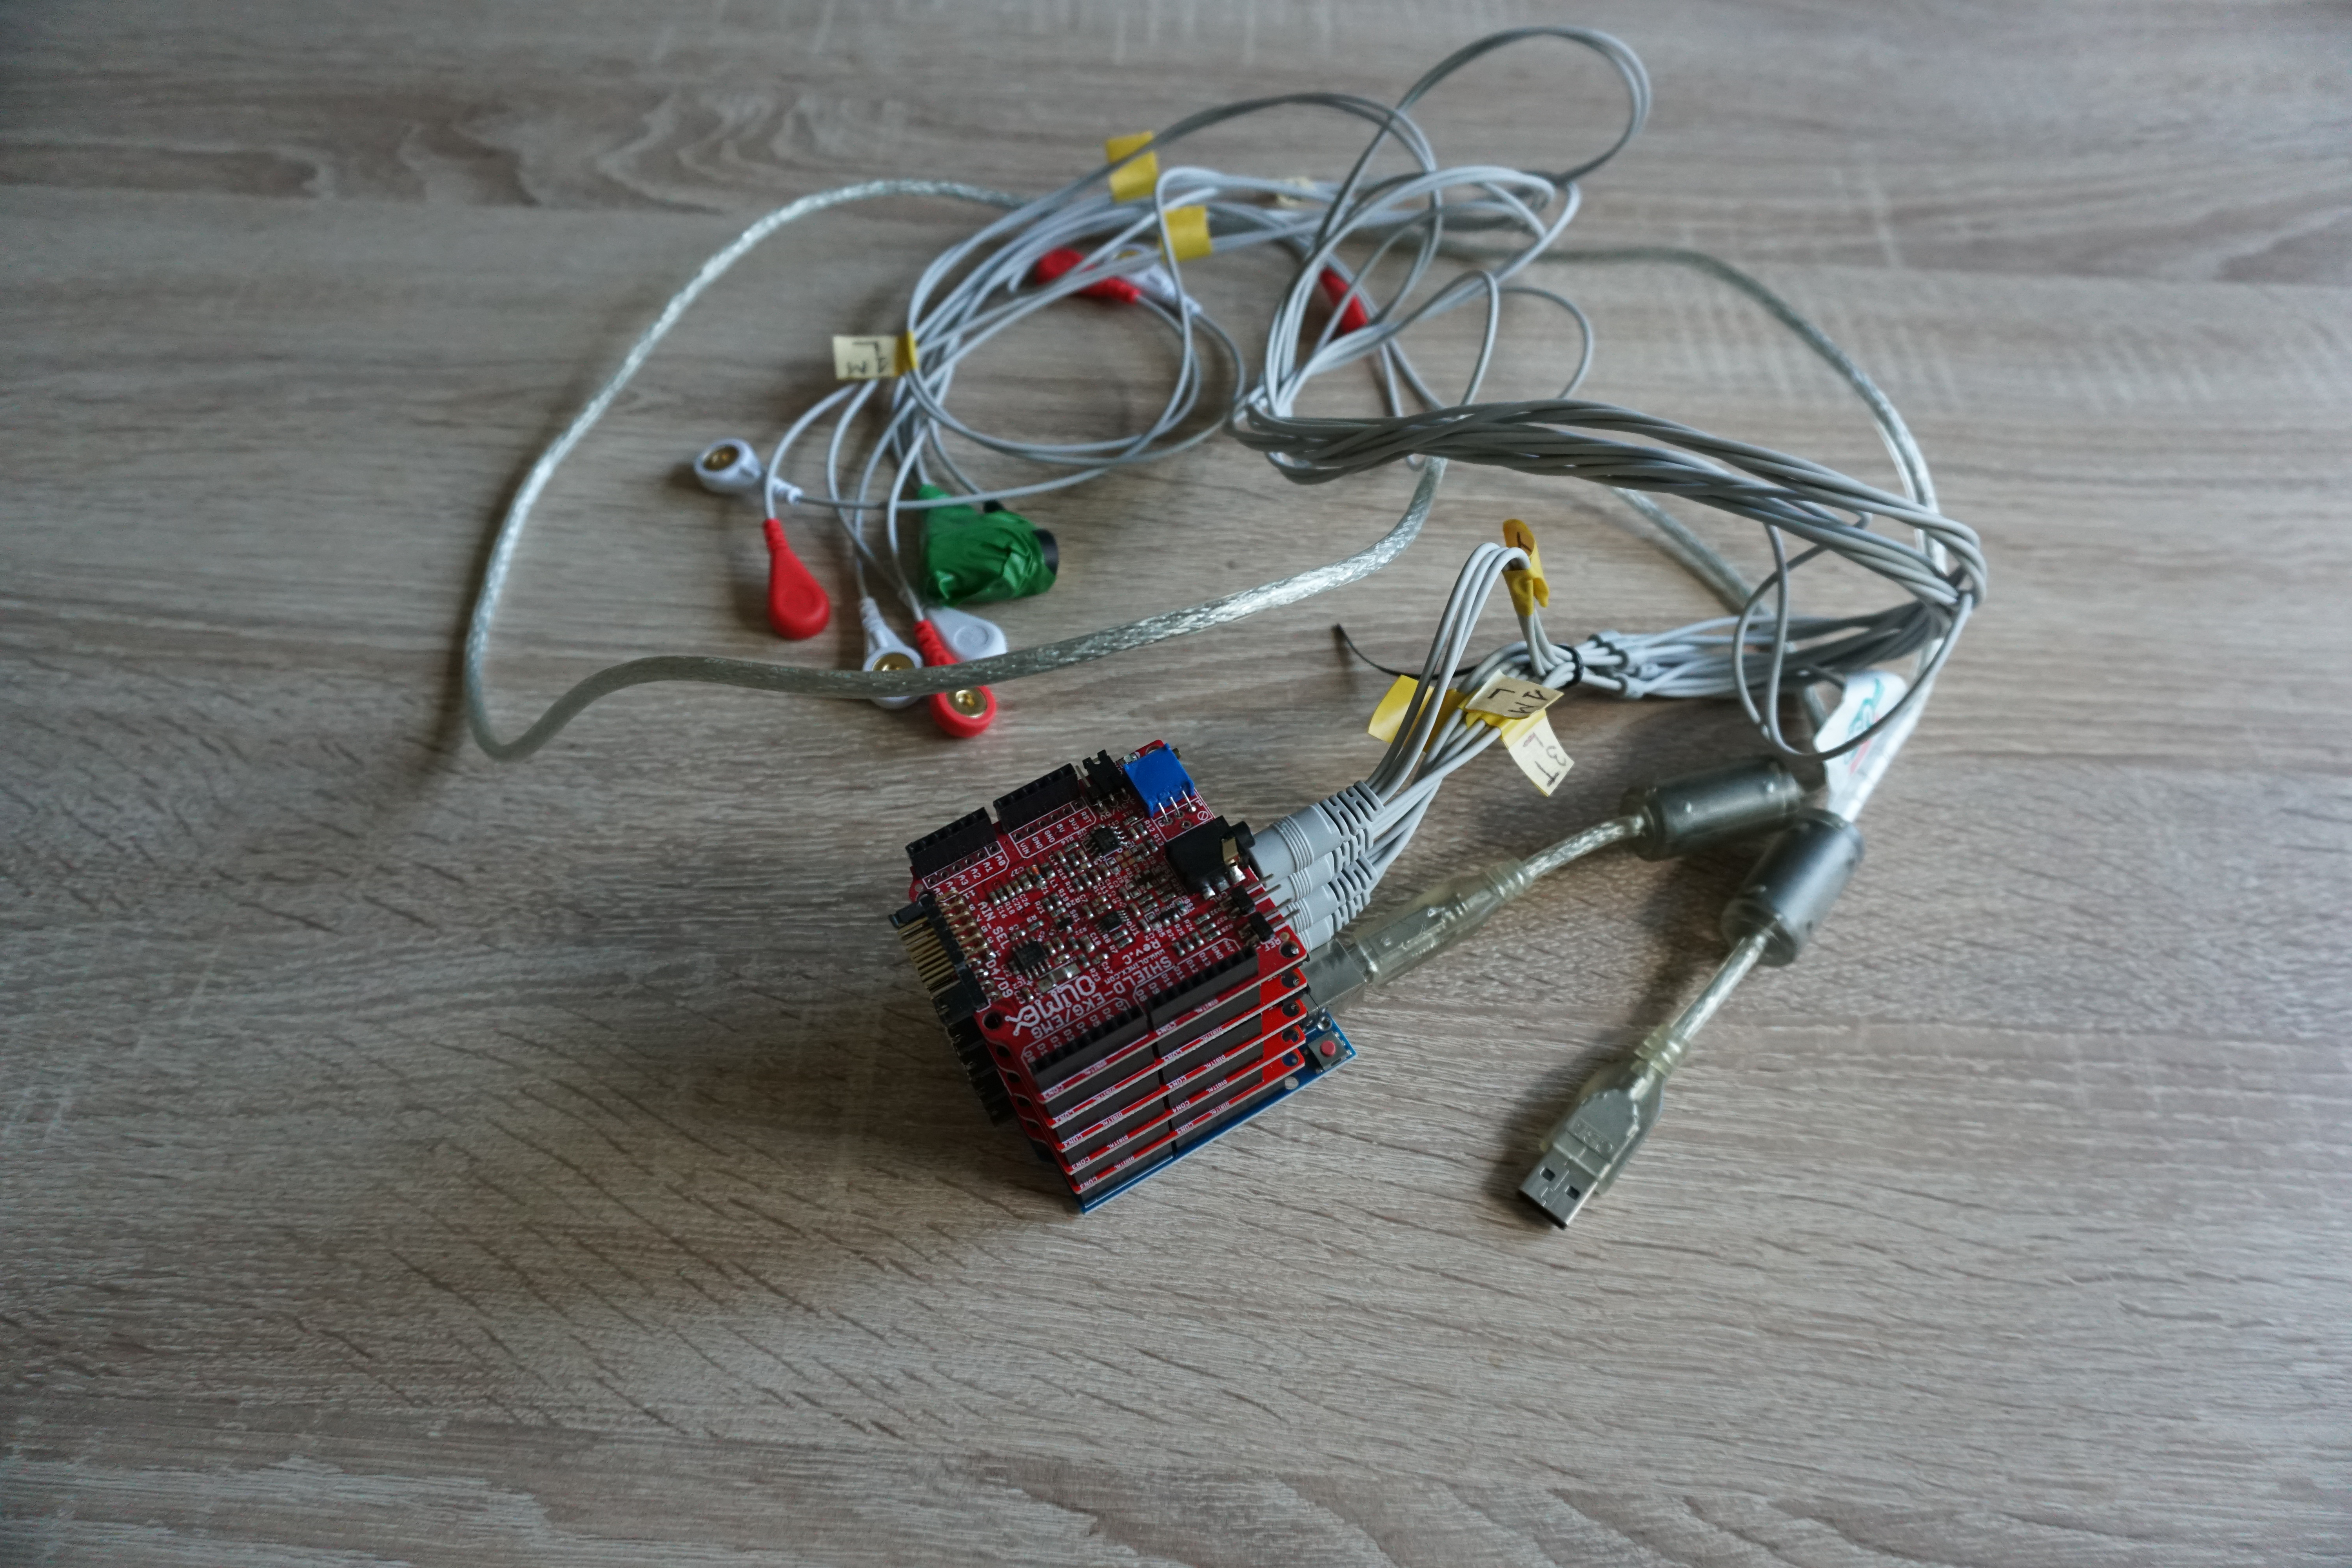
\includegraphics[width=0.5\textwidth]{src/media/hardware/real-emg-top.JPG}
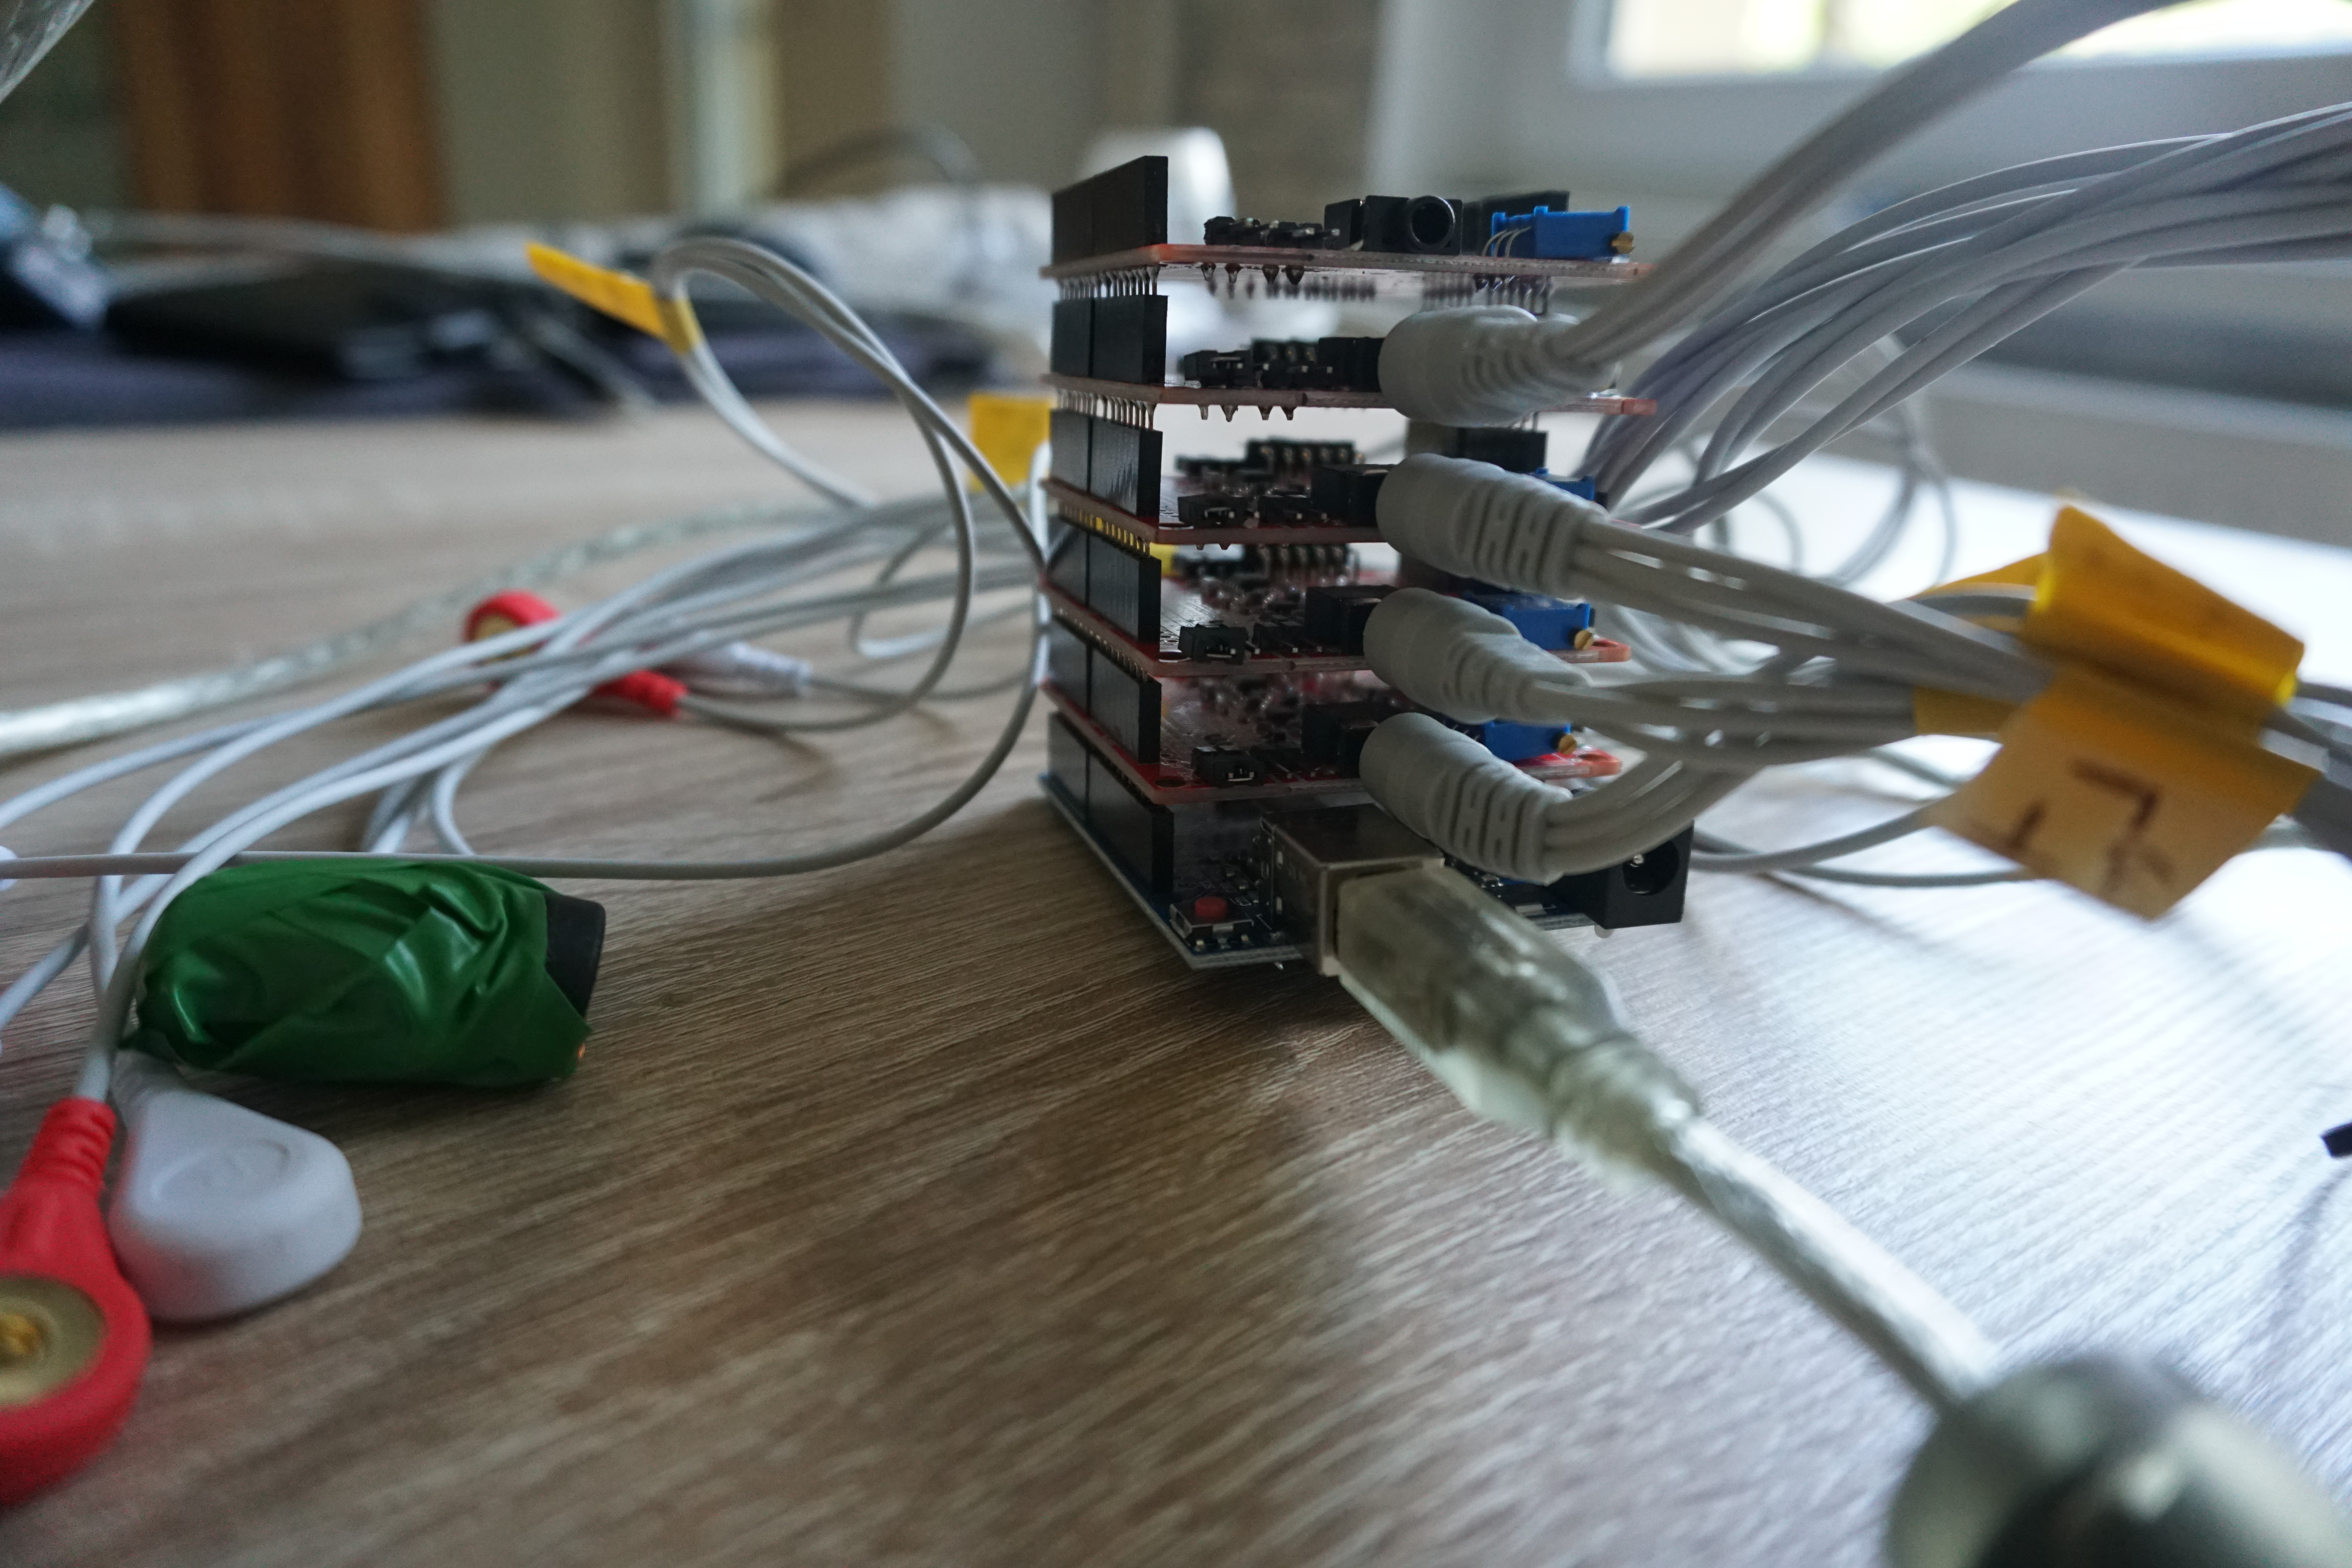
\includegraphics[width=0.5\textwidth]{src/media/hardware/real-emg-side.JPG}
\caption{Prototype of EMG-Shields with Arduino Uno}
\label{image:real-emg}
\end{figure}


\section{Software}
\label{sec:software}